\section{Series}
	\subsection{Divergence Test}
	If the series is:
	$$\sum^{\infty}_{n=0}a_n$$
	if
	$$\lim_{n\to\infty}a_n \neq 0$$
	then the series diverges. 
	
	\subsection{Geometric Series}
	Geometry series takes the form of:
	\begin{equation}
	\sum^{\infty}_{n=0}ar^n
	\end{equation}
	
	\noindent The series only converges to 
	\begin{equation}
	\frac{a}{1-r}
	\end{equation}
	if and only if $|r|<1$
	
	\subsection{p-series}
	p-series takes the form of
	\begin{equation}
	\frac{1}{n^p}
	\end{equation}
	
	\noindent p-series only converges when $p>1$
	
	\subsection{Comparison Test}
	\begin{theorem}{}{}
	If there are two series 
	\begin{multicols}{2}\noindent 
	\begin{equation}
	\displaystyle\sum^\infty_{n\to\infty}a_n
	\end{equation}
	\begin{equation}
	\displaystyle\sum^\infty_{n\to\infty}b_n
	\end{equation}
	\end{multicols}
	
	\noindent and
	
	$$a_n\ \text{is always bigger than or equal to}\ b_n\ as\ n\to\infty$$
	\begin{center}
	or
	\end{center}
	$$b_n\ \text{is always smaller than or equal to}\ a_n\ as\ n\to\infty$$
	
	\noindent if $\displaystyle\sum^{\infty}_{n\to\infty}a_n$ converges then $\displaystyle\sum^{\infty}_{n\to\infty}b_n$ must also converge.\\
	\noindent if $\displaystyle\sum^{\infty}_{n\to\infty}b_n$ diverges then $\displaystyle\sum^{\infty}_{n\to\infty}a_n$ must also diverge.
	\begin{tiny}
	\noindent Its really similar to the comparison test of infinite integral.
	\end{tiny}
	\end{theorem}
	
	\begin{theorem}{}{}
	\label{comparison_test}
	The bigger the denominator gets, the smaller the value become
	\end{theorem}
	
	 
	\begin{simple}{}{}
	Find if
	$$\frac{1}{x^2+x+2}$$
	will converge.
	
	\begin{enumerate}
	\item Think of a similar sequence that might help
	\begin{tiny}
	It takes a lot of practice.
	\end{tiny}\\
	In this case we will use $\frac{1}{x^2}$ for converge
	
	\item Make sure it is actually smaller/bigger than the series of interest.\\
	We need $\frac{1}{x^2}$ to be smaller than $\frac{1}{x^2+x+2}$
	
	\begin{center}
	    \begin{tikzpicture}
    	\begin{axis}[xmax=20, xmin=0,ymin=0,ymax=0.6, axis lines=middle]
    	\addplot[samples=50, domain=0:20, color=red]{1/(x^2+x+2)}
    	node[pos=0.1, right]{$f(x)=\frac{1}{n^2+n+2}$};
    	
    	\addplot[samples=50, domain=0:20, color=blue]{1/(x^2)}
    	node[pos=0.25, right]{$g(x)=\frac{1}{n^2}$};
    	\end{axis}
    	\end{tikzpicture}
	\end{center}
	
	In this case, $\frac{1}{n^2}$ is always bigger than $\frac{1}{n^2+n+2}$
	
	\item Since $\frac{1}{x^2}$ converges$_{p-series}$
	, $\frac{1}{x^2+x+2}$ must also converge.
	\end{enumerate}
	\end{simple}
	
	\begin{example}{}{}
	Find if
	$$\sum^\infty_{n=0}\frac{1}{\ln{n}}$$
	converges.
	
	\begin{enumerate}
	    \item We can use $\frac{1}{n}$ to compare
	    \item $\frac{1}{n}$ is always going to be smaller than $\frac{1}{\ln{n}}$
	    \begin{center}
	        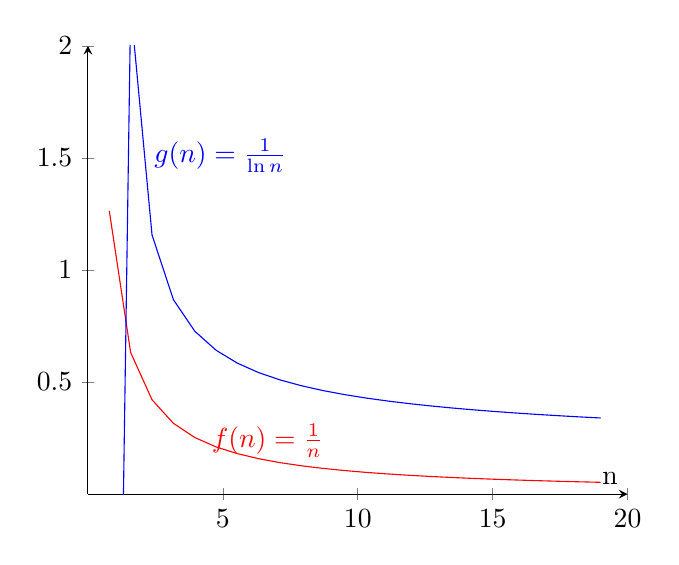
\begin{tikzpicture}
	            \begin{axis}[axis lines=middle, xmin=0, xmax=20, ymin=0, ymax=2, xlabel=n]
	                    \addplot[domain=0:19, color=red]{1/x}
	                    node[pos=0.2, right]{$f(n)=\frac{1}{n}$};
	                    \addplot[domain=0:19, color=blue]{1/ln(x)}
	                    node[pos=0.3, right]{$g(n)=\frac{1}{\ln{n}}$};
	            \end{axis}
	        \end{tikzpicture}
	    \end{center}
	    
	    \noindent $\frac{1}{\ln{n}}$ is always bigger than $\frac{1}{n}$ in the longer run.
	    
	    \item $\frac{1}{n}$ diverges$_p-series$, so $\frac{1}{\ln{n}}$ has to diverge.
	\end{enumerate}
	\end{example}
	
	\begin{example}{}{}
	Find if
	$$\sum^\infty_{n=0}\frac{1}{0.789^n+0.789^{n-1}+0.789^{n-2}+\ldots{}}$$
	converges
	\begin{enumerate}
	    \item Compare it to the equation:
	    $$\frac{1}{0.789^n}$$
	    \item Using theorem 2 stated above, we can conclude $\frac{1}{0.789^n+0.789^{n-1}+0.789^{n-2}+\ldots{}}$ is always smaller than $\frac{1}{0.789^n}$ in the long run.
	    \item $\displaystyle\sum^\infty_{n=0}\frac{1}{0.789^n}$ can be written in the form of a geometric series: 
	    \begin{align*}
	        \sum^\infty_{n=0}\frac{1}{0.789^n}&=\sum^\infty_{n=0}1*\frac{1}{0.789^n}_{Hint: \sum^\infty_{n=0}a*r^n}\\
	        &=\sum^\infty_{n=0}1*\left(\frac{1}{0.789}\right)^n
	    \end{align*}
	    In this case $$a=1,\ \ r=\frac{1}{0.789}$$\\
	    $|r|$ is smaller than 1, subbing variables into $\displaystyle\frac{a}{1-r}$
	    $$\sum^\infty_{n=0}\frac{1}{0.789^n}=\frac{1}{1-0.789}\approx4.73$$
	    
	    \item Since $\sum^\infty_{n=0}\frac{1}{0.789^n}$ converges, $\sum^\infty_{n=0}\frac{1}{0.789^n+0.789^{n-1}+0.789^{n-2}+\ldots{}}$ must also converge
	\end{enumerate}
	\end{example}
	
	\subsection{Integral Test}
	Given $f(n)=a_n$ for all integer values of n and f(x) is a continuous and decreasing function.
	\begin{theorem}{}{integral_test}
    	if $\displaystyle\int^\infty_cf(x)$ converges then $\displaystyle\sum^{\infty}_{n=0}a_n$ will converge.\\
    	if $\displaystyle\int^\infty_cf(x)$ diverges then $\displaystyle\sum^{\infty}_{n=0}a_n$ will diverge.\\
    	c can be any finite integer
	\end{theorem}
	
	\begin{simple}{}{}
	Find if
	$$\frac{1}{n^2}$$
	converges?\\
	
	We can take a look at the integral:
	\begin{align*}
	    \int^\infty_1\frac{1}{n^2}dn&=\lim_{t\to\infty}\int^t_0\frac{1}{n^2}dn\\
	    &=\lim_{t\to\infty}-\left.\frac{1}{n}\right|^t_1\\
	    &=\lim_{t\to\infty}-\left(\frac{1}{t}-\frac{1}{1}\right)\\
	    &=-\left(0-1\right)\\
	    &=1
	\end{align*}
	
	Since the integral $\displaystyle\int^\infty_1\frac{1}{n^2}$ converges, the series will converge.
	\end{simple}
	
	The challenge to this kind of questions is to solve the integral, not apply integral test.
	
	\subsection{Alternating Series}
	\begin{theorem}{}{}
	    If a series takes one of these forms:
	    \begin{multicols}{2}
	    \noindent\begin{equation}
	        \sum^\infty_{n=0}(-1)^n a_n
	    \end{equation}
	    \begin{equation}
	        \sum^\infty_{n=0}(-1)^{n+1}a_n
	    \end{equation}
	    \end{multicols}
	    
	    and $a_n$ is a constantly decreasing towards 0. \\
	    The series is going to converge.
	\end{theorem}
	
	In simpler words, the requirements for an alternating series are:
	\begin{enumerate}
	    \item Constantly alternating between positive and negative
	    \item $\displaystyle\lim_{n\to\infty}=0$
	    \item $a_n\geq a_{n+1}$
	\end{enumerate}
	
	\begin{simple}{}{}
	Will 
	$$\sum^\infty_{n=0} \frac{(-1)^nn}{n^3}$$
	converge?
	
	Solution:
	We will check if it satisfies the conditions of an alternating series.
	\begin{enumerate}
	    \item The function is going to switch between positive and negative
	    \item $\displaystyle\lim_{n\to\infty}\frac{n}{n^3}=0$
	    \item $\dfrac{1}{(n+1)^2}\leq\dfrac{1}{n^2}$
	\end{enumerate}
	
	The series qualifies for all three conditions, therefore it is an alternating series and must converge.
	\end{simple}
	
	\subsection{Ratio Test}
	\begin{theorem}{Absolute Convergence}{}
	    When $\displaystyle\sum^\infty_{n=0}\left|a_n\right|$ converges, $\displaystyle\sum^\infty_{n=0}a_n$ must also converge.
	\end{theorem}
	\begin{theorem}{Conditional Convergence}{}
	    When $\displaystyle\sum^\infty_{n=0}a_n$ converges, $\displaystyle\sum^\infty_{n=0}\left|a_n\right|$ might not converge.
	\end{theorem}
	
	\begin{theorem}{}{}
	    Given a function in the form:
	    $$\sum^\infty_{n=0}a_n$$
	    
	    Find 
	    \begin{equation}
	        \lim_{n\to\infty}\left|\frac{a_{n+1}}{a_n}\right|
	    \end{equation}
	    
	    There are three possible outcomes
        \begin{enumerate}
            \item The limit is smaller than 1$_{including\ 0}$, the series is absolute convergent.
            \item The limit is equal to 1, the test is inconclusive.
            \item the limit is greater than 1$_{including\ \infty}$, the series diverges
        \end{enumerate}
	\end{theorem}
	
	Ratio test is really helpful when you have exponents or factorial
	
	\subsection{Root Test}
	
	This test is really similar to ratio test.
	
	\begin{theorem}{}{}
	    Given a function in the form:
	    $$\sum^\infty_{n=0}a_n$$
	    
	    Find 
	    \begin{equation}
	        \lim_{n\to\infty}\sqrt[n]{\left|a_n\right|}
	    \end{equation}
	    
	    There are three possible outcomes
        \begin{enumerate}
            \item The limit is smaller than 1$_{including\ 0}$, the series is absolute convergent.
            \item The limit is equal to 1, the test is inconclusive.
            \item the limit is greater than 1$_{including\ \infty}$, the series diverges
        \end{enumerate}
	\end{theorem}
	
	\subsection{Checklist of Tests}
	\begin{enumerate}
	    \item Comparison Test (p-series/geometric series)
	    \item Alternating Series Test ($(-1)^n$)
	    \item Ratio Test (exponents or factorial)
	    \item Integral Test (decreasing, positive and continuous)
	    \item Divergent Test (Last resort)
	\end{enumerate}
	
	\subsection{Power Series}
	\begin{theorem}{}{}
	A power series centered at $x_0$ is a series takes the form:
	\begin{equation}
	    \sum^\infty_{n=0}c_n(x-x_0)^n
	\end{equation}
	\end{theorem}
	
	Unlike before, power series has a variable. x can be any value and it will influence whether the power series converges.
	
	\begin{simple}{}{}
	We can take a look at 
	$$\sum^\infty_{n=0}\frac{(x)^n}{2^n}$$
	
    If we let x=5
    
    $$\sum^\infty_{n=0}\frac{5^n}{2^n}=\sum^\infty_{n=0}\left(\frac{5}{2}\right)^n$$
    
    It becomes a geometric series. Since $|r|$ is bigger than 1, the series diverges.\\
    
    If we let x=1
    $$\sum^\infty_{n=0}\frac{1^n}{2^n}=\sum^\infty_{n=0}\left(\frac{1}{2}\right)^n$$
    
    In this case $|r|$ is smaller than 1, the series converges.
    
    Note that not all power series are this simple!
	\end{simple}
	
	\begin{theorem}{}{}
	There are three possible cases of x that will convergence the series:
	\begin{enumerate}
	    \item Only converge at $x_0$
	    \item Converges within an interval
	    \item Converges for all x
	\end{enumerate}
	It should be noted the series will always converge at $x_0$.
	\end{theorem}
	
	When you are finding interval of convergence for some series, always try ratio test.
	
	\begin{simple}{}{}
	Find the interval of convergence for
	$$\sum^\infty_{n=0}\frac{x^n}{n*3^n}$$
	
    Solution:
    \begin{align*}
    \displaystyle
        \lim_{n\to\infty}\left|\frac{\frac{x^{n+1}}{(n+1)3^{n+1}}}{\frac{x^n}{n*3^n}}\right|&=\lim_{n\to\infty}\left|\frac{x*n}{(n+1)3}\right|\\
        &=\lim_{n\to\infty}\left|\frac{x}{3}\frac{n}{n+1}\right|\\
        &=\left|\frac{x}{3}\right|\\
    \end{align*}
    
    $\left|\dfrac{x}{3}\right|$ has to be smaller than 1 for the series will converge.
    
    \begin{align*}
        \left|\frac{x}{3}\right|&<1\\
        -1<\frac{x}{3}&<1\\
        -3<x&<3
    \end{align*}
    
    Now that we know the radius of convergence, we need to find if the boundaries converge.
    
    \begin{multicols}{2}
    When x=-3:
    \begin{align*}
        &=\sum^\infty_{n=0}\frac{(-3)^n}{n*3^n}\\
        &=\sum^\infty_{n=0}\frac{(-1)^n3^n}{n*3^n}\\
        &=\sum^\infty_{n=0}(-1)^n\frac{1}{n}
    \end{align*}
    {Alternating series, the series converges when x=-3}\\
    When x=3:
    \begin{align*}
        &=\sum^\infty_{n=0}\frac{(3)^n}{n*3^n}\\
        &=\sum^\infty_{n=0}\frac{1}{n}
    \end{align*}
    
    p-series, the series diverges at x=3\\\\
    \end{multicols}
    
    The interval of convergence is $[-3<x<3)$
	\end{simple}
	
	\noindent Geometric series can be considered as a power series centered at 0 and all constant $c_n=a$.$$\sum^\infty_{n=0} ar^n=\sum^\infty_{n=0}c_nx^n$$
	
	\begin{simple}{}{}
	    Express 
	    $$f(x)=\frac{3}{1+x^3}$$
	    as a series.\\
	    Solution:
	    \begin{align*}
	        f(x)=\frac{3}{1+x^3}&=\frac{3}{1-(-x^3)}\\
	        &=\sum^\infty_{n=0}3(-x^3)^n
	    \end{align*}
	\end{simple}
	
	\subsection{Term by Term Differentiation and Integration}
	\begin{theorem}{}{}
	\begin{equation}
	    f(x)=\sum^\infty_{n=0}c_n(x-x_0)^n
	\end{equation}
	\begin{equation}
	    f'(x)=\sum^\infty_{n=1}c_n*n*(x-x_0)^{n-1}
	\end{equation}
	\begin{equation}
	    \int f(x)dx=\sum^\infty_{n=1}c_n\frac{(x-x_0)^{n+1}}{n+1}+C
	\end{equation}
	
	P.S. $f(0)=C$ and remember n=1 for differentiation of series.
	\end{theorem}
	
	\subsection{Taylor Series}
	\subsubsection{Function to Taylor Series}
	\begin{theorem}{}{}
	Taylor series of f(x) is:
	\begin{equation}{}{}
	    f(x)=\sum^\infty_{n=0}\frac{f^n(x_0)}{n!}(x-x_0)^n
	\end{equation}
	\end{theorem}
	
	\begin{simple}{}{}
	    $$f(x)=\sin{(x)}$$
	    Find f(x) represented using power series centered at $x_0=\dfrac{\pi}{2}$
	    
	    \begin{multicols}{2}
	    \begin{center}
	        $f(x)=\sin{(x)}$\\
    	    $f'(x)=\cos{(x)}$\\
    	    $f''(x)=-\sin{(x)}$\\
    	    $f^3(x)=-\cos{(x)}$\\
    	    $f^4(x)=\sin{(x)}$\\
    	    $f(\frac{\pi}{2})=1$\\
    	    $f'(\frac{\pi}{2})=0$\\
    	    $f''(\frac{\pi}{2})=-1$\\
    	    $f^3(\frac{\pi}{2})=0$\\
    	    $f^4(\frac{\pi}{2})=1$
	    \end{center}
	    \end{multicols}
	    
	    \begin{align*}
	        f(x)&=\sin{(\frac{\pi}{2})}\\
	        &+\dfrac{\cos(\frac{\pi}{2})}{1!}\left(x-\frac{\pi}{2}\right)\\
	        &+\dfrac{-\sin{(\frac{\pi}{2})}}{2!}\left(x-\frac{\pi}{2}\right)^2\\
	        &+\frac{-\cos{(\frac{\pi}{2})}}{3!}\left(x-\frac{\pi}{2}\right)^3\\
	        &+\frac{\sin{(x)}}{4!}\left(x-\frac{\pi}{2}\right)^4 \ldots{}\\
	        f(x)&=1+0-\frac{1}{2}\left(x-\frac{\pi}{2}\right)^2+\frac{1}{24}\left(x-\frac{\pi}{2}\right)^4\ldots
	    \end{align*}
	    
	    By looking at the pattern we observe that
	    $$f(x)=\sum^\infty_{n=0}\dfrac{(-1)^n}{(2n)!}\left(x-\dfrac{\pi}{2}\right)^{2n}$$
	\end{simple}
	\subsubsection{Visualization of Taylor Series}
	You don't need to know this for the course, but its pretty fun.
	\begin{align*}
	    f_0(x)&=1\\
	    f_1(x)&=1-\frac{1}{2}\left(x-\frac{\pi}{x}\right)^2\\
	    f_2(x)&=1-\frac{1}{2}\left(x-\frac{\pi}{x}\right)^2+\frac{1}{24}\left(x-\frac{\pi}{2}\right)^4\\
	    f_3(x)&=1-\frac{1}{2}\left(x-\frac{\pi}{x}\right)^2+\frac{1}{24}\left(x-\frac{\pi}{2}\right)^4-\frac{1}{720}\left(x-\frac{\pi}{2}\right)^6\\
	    f_4(x)&=1-\frac{1}{2}\left(x-\frac{\pi}{x}\right)^2+\frac{1}{24}\left(x-\frac{\pi}{2}\right)^4-\frac{1}{720}\left(x-\frac{\pi}{2}\right)^6+\frac{1}{40320}\left(x-\frac{\pi}{2}\right)^8
	\end{align*}
	
	\begin{multicols}{2}
	\begin{center}
	
	    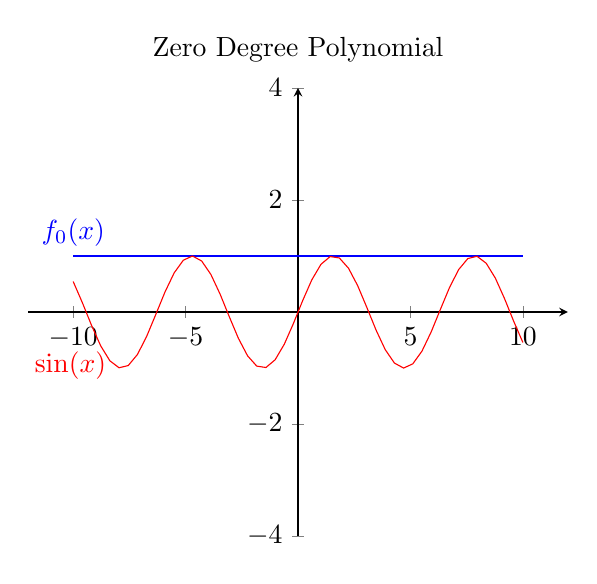
\begin{tikzpicture}
	    \begin{axis}[ymax=4, ymin=-4, xmin=-12, xmax=12, axis lines=middle, title=Zero Degree Polynomial]
	        \addplot[color=blue, domain=-10:10, samples=2]{1}node[anchor=south, pos=0]{$f_0(x)$};
	        \addplot[color=red, domain=-10:10,
	        samples=50]{sin(deg(x))}node[anchor=east, pos=0.1]{$\sin(x)$};
	    \end{axis}
	\end{tikzpicture}
    
	
	    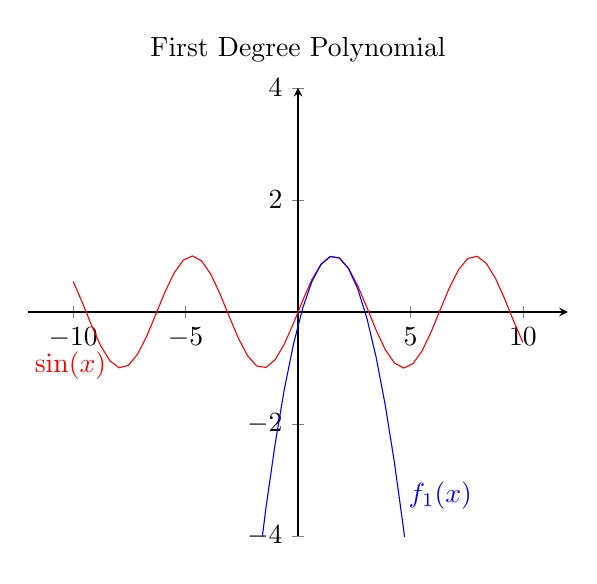
\begin{tikzpicture}
	    \begin{axis}[ymax=4, ymin=-4, xmin=-12, xmax=12,axis lines=middle, title=First Degree Polynomial]
	    \addplot[color=red, domain=-10:10,
	    samples=50]{sin(deg(x))}node[anchor=east, pos=0.1]{$\sin(x)$};
	    \addplot[color=blue, domain=-10:10, samples=50]{1-(x-pi/2)^2/2}node[pos=0.7, anchor=west]{$f_1(x)$};
	    \end{axis}
	    \end{tikzpicture}\\
	
	    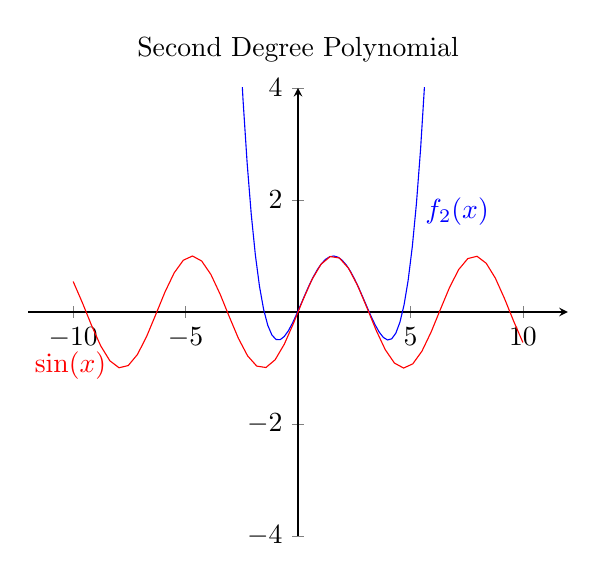
\begin{tikzpicture}
	    \begin{axis}[ymax=4, ymin=-4, xmin=-12, xmax=12, axis lines=middle, title=Second Degree Polynomial]
	        \addplot[color=blue, domain=-3:6, samples=50]{1-(x-pi/2)^2/2+(x-pi/2)^4/24}node[anchor=west, pos=0.77]{$f_2(x)$};
	        \addplot[color=red, domain=-10:10,
	        samples=50]{sin(deg(x))}node[anchor=east, pos=0.1]{$\sin(x)$};
	    \end{axis}
	\end{tikzpicture}\\
	
	
	    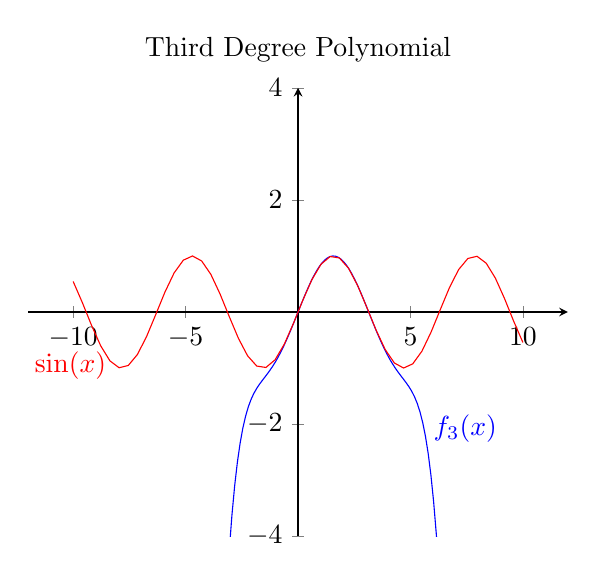
\begin{tikzpicture}
	    \begin{axis}[ymax=4, ymin=-4, xmin=-12, xmax=12, axis lines=middle, title=Third Degree Polynomial]
	        \addplot[samples=100, color=blue, domain=-5:7]{1-(x-pi/2)^2/2+(x-pi/2)^4/24-(x-pi/2)^6/720}
	        node[anchor=west, pos=0.85]{$f_3(x)$};
	        \addplot[color=red, domain=-10:10,
	        samples=50]{sin(deg(x))}node[anchor=east, pos=0.1]{$\sin(x)$};
	    \end{axis}
	\end{tikzpicture}\\
	
	\end{center}
	\end{multicols}
	
	\begin{center}
	    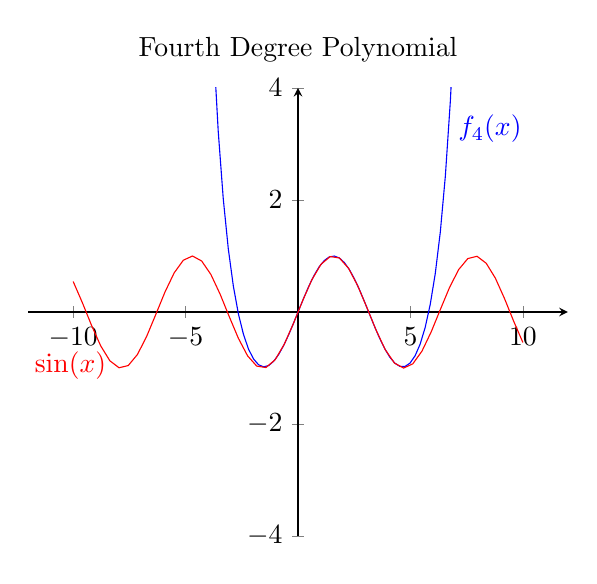
\begin{tikzpicture}
	    \begin{axis}[ymax=4, ymin=-4, xmin=-12, xmax=12, axis lines=middle, title=Fourth Degree Polynomial]
	        \addplot[samples=50, color=blue, domain=-4:7]{1-(x-pi/2)^2/2+(x-pi/2)^4/24-(x-pi/2)^6/720+(x-pi/2)^8/40320}node[pos=0.9, anchor=west]{$f_4(x)$};
	        \addplot[color=red, domain=-10:10,
	        samples=50]{sin(deg(x))}node[anchor=east, pos=0.1]{$\sin(x)$};
	    \end{axis}
	\end{tikzpicture}
	\end{center}
	
	\noindent As the number of Taylor polynomial terms increases, the series approaches the original function.
	
	\begin{theorem}{}{}
	    Maclaurin Series are Taylor Series centered at x=0
	    \begin{equation}
	        \sum^\infty_{n=0}\frac{f^n(0)}{n!}x^n
	    \end{equation}
	\end{theorem}
	
	\subsection{Estimation using Series}
	\subsubsection{Alternating Series}
	
	Let's do another visualization:\\
    \begin{simple}{}{}
        Let $S_N$ denote the sum of N terms of the alternating series. We will try to approximate:
        $$\sum^\infty_{n=0}(-1)^n\frac{1}{2^n}$$
        \begin{align*}
            S_0&=1\\
            S_1&=1-\frac{1}{2}\\
            S_2&=1-\frac{1}{2}+\frac{1}{4}\\
            S_3&=1-\frac{1}{2}+\frac{1}{4}-\frac{1}{8}\\
            S_4&=1-\frac{1}{2}+\frac{1}{4}-\frac{1}{8}+\frac{1}{16}\\
            S_5&=1-\frac{1}{2}+\frac{1}{4}-\frac{1}{8}+\frac{1}{16}-\frac{1}{32}\\
            S_6&=1-\frac{1}{2}+\frac{1}{4}-\frac{1}{8}+\frac{1}{16}-\frac{1}{32}+\frac{1}{64}\\
        \end{align*}
        \begin{center}
            \begin{tikzpicture}
            \begin{axis}[clip=false, axis lines=middle, xmin=0, xmax=7, ymax=1.2, ymin=0, xlabel=n, ylabel=Sum, title=Visualization of Alternating Series]
            \addplot[only marks, color=blue]
            coordinates{
            (0, 1)
            (1, 1/2)
            (2, 3/4)
            (3, 5/8)
            (4, 11/16)
            (5, 21/32)
            (6, 43/64)
            };
            \addplot[color=red, domain=0:7]{2/3}node[anchor=west]{$\frac{2}{3}$};
            \end{axis}
            \end{tikzpicture}
        \end{center}
        
        As you can verify, the series sums to $\frac{2}{3}$.
    \end{simple}
	
	\begin{theorem}{}{}
	    \indent Let S represent the sum of an alternating series.
	    $$\sum^\infty_{n=0}(-1)^na_n$$
	    Let $R_N$ represent the remainder of the series so that $R_N=S-S_N$. 
        \begin{equation}
            \left|R_N\right|\leq a_{n+1}
        \end{equation}
	\end{theorem}
	
	In simpler words, the distance from $S_N$ to series value is always smaller than distance to $S_{N+1}$.
	
	\subsubsection{Taylor Series}
	\begin{theorem}{}{}
	Let S denote the value of f(x) at x(Top dot).\\
	\begin{multicols}{2}
	\begin{center}
	    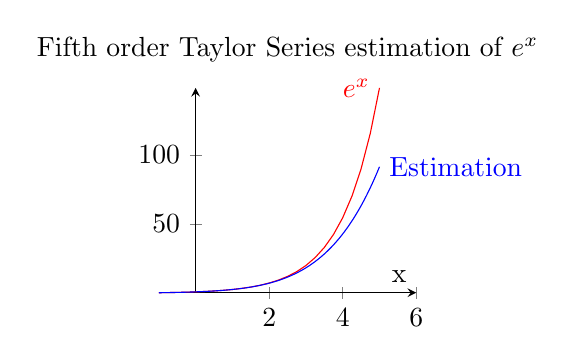
\begin{tikzpicture}
    	\begin{axis}[width=0.4\textwidth, clip=false, axis lines=middle, xmin=-1, xmax=6, xlabel=x, title=Fifth order Taylor Series estimation of $e^x$]
    	\addplot[color=red, domain=-1:5]{e^x}node[anchor=east]{$e^x$};
    	\addplot[color=blue, samples=100, domain=-1:5]{1+x+(x^2)/2+(x^3)/6+(x^4)/24+(x^5)/120}node[anchor=west]{Estimation};
    	\end{axis}
    	\end{tikzpicture}
	\end{center}
	\begin{center}
	    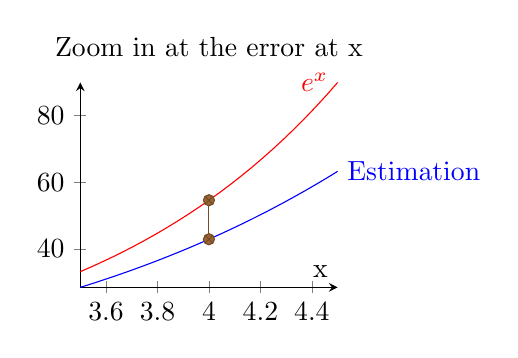
\begin{tikzpicture}
    	\begin{axis}[clip=false, width=0.4\textwidth, axis lines=middle, xmin=3.5, xmax=4.5, xlabel=x, title=Zoom in at the error at x=4]
    	\addplot[color=red, domain=3.5:4.5]{e^x}node[anchor=east]{$e^x$};
    	\addplot[color=blue, samples=100, domain=3.5:4.5]{1+x+(x^2)/2+(x^3)/6+(x^4)/24+(x^5)/120}node[anchor=west]{Estimation};
    	\addplot coordinates{
    	(4, 54.5981)
    	(4, 42.8666666)
    	};
    	\end{axis}
    	\end{tikzpicture}
	\end{center}
	\end{multicols}
	
	Let $S_N$ represent the sum of the series evaluated at x for N terms.(Bottom dot)\\
	Let $R_N$ represent the error such that $R_n=S-S_N$(The line connecting two dots).
	
	\begin{equation}
	        \left|R_n(x)\right|\leq \frac{M}{(n+1)!}|x-x_0|^{n+1}
	    \end{equation}
	    Where M is the maximum value of f'(x) between x and $x_0$
	\end{theorem}
	\begin{proof}
	Bruh, just trust me.
	\end{proof}
	
	\begin{theorem}{Taylor Series Error Bound}{}
	    To prove that a series is equal to a function:
	    \begin{equation}
	        \lim_{n\to\infty}\frac{M}{(n+1)!}(x-x_0)^{n+1}=0
	    \end{equation}
	    and 
	    \begin{equation}
	        -\lim_{n\to\infty}\frac{M}{(n+1)!}(x-x_0)^{n+1}=0
	    \end{equation}
	\end{theorem}
	
	\begin{proof}
    Using theorem Taylor Series Error Bound:
    $$\left|R_n(x)\right|\leq \frac{M}{(n+1)!}|x-x_0|^{n+1}$$
    We can conclude:
    $$-\frac{M}{(n+1)!}|x-x_0|^{n+1}\leq R_n(x)\leq \frac{M}{(n+1)!}|x-x_0|^{n+1}$$
    
    \noindent If both sides equal to 0 as n approaches infinity, it forces $R_n(x)$ to be equal to zero according to squeezing theorem. If there is no error, the series and the function are equivalent. 
	\end{proof}
	
	\begin{simple}{}{}
	    Prove the Taylor series of $\sin{(x)}$ is 
	    $$f(x)=\sum^\infty_{n=0}\dfrac{(-1)^n}{(2n)!}\left(x-\dfrac{\pi}{2}\right)^{2n}$$
	    
	    Solution:\\
	    $f'(x)=\cos{(x)}$
	    We know that the maximum for a cosine function is going to be 1, therefore, M=1.
	    
	    \begin{align*}
	        \lim_{n\to\infty}\frac{1}{(n+1)!}|x-x_0|^{n+1}&=\lim_{n\to\infty}\frac{x^n}{n!}\\
	        &=0
	    \end{align*}
	    
	    Similar calculation can be perform on $-\frac{M}{(n+1)!}|x-x_0|^{n+1}$.
	    
	    Since both conditions are satisfied, this Taylor series is equivalent to the function.
	\end{simple}
	
	